\documentclass[11pt]{article}

\usepackage[a4paper,margin=26mm]{geometry}
\usepackage[T1]{fontenc}
\usepackage[utf8]{inputenc}
\usepackage{lmodern}
\usepackage{microtype}
\usepackage{amsmath,amssymb,mathtools}
\usepackage{booktabs}
\usepackage{enumitem}
\usepackage{graphicx}
\usepackage[round,authoryear]{natbib}
\usepackage[hidelinks]{hyperref}
\hypersetup{
  pdftitle={From Orienting Signals to Self-Pointers},
  pdfauthor={Gunnar Zarncke},
  pdfsubject={Self-pointers, recirculation, agency, and self-binding}
}

\setlist{nosep,leftmargin=*}
\setlength{\parindent}{1.2em}
\setlength{\parskip}{0.25em}

\newcommand{\E}{\mathbb{E}}
\newcommand{\I}{\mathbb{I}}
\newcommand{\R}{\mathbb{R}}
\newcommand{\Pp}{\mathbb{P}}

\title{\textbf{From Orienting Signals to Self-Pointers}\\
\large A Minimal Computational Experiment on Self-Binding}
\author{Gunnar Zarncke}
\date{September 2026}

\begin{document}
\maketitle

\begin{abstract}
A model sees two identical bodies. Only one generates its internal signals. Can it learn which body is ``me'' without being told? We call the answer a \emph{self-pointer}: a persistent latent that marks one body as the source of privileged cues and the locus of control-relevant consequences. We test this in matched counterfactual worlds---same visible history, opposite action labels---with ablatable cues (orienting response, efference copy, proprioception) and optional recirculation of a recurrent bottleneck into object tokens. Ten-seed learning curves to 300 updates show vision and proprioception at chance, orienting-related conditions crossing a delayed transition to ${>}93\%$ accuracy, and cue combinations learning slightly faster early on. Task accuracy alone does not prove a reusable self-pointer; probes and causal state swaps are the stronger tests. This is not a consciousness paper. It asks whether organism-centered signals can ground ``which body is mine?'' in world-model state.
\end{abstract}

\section{Introduction}

Imagine two identical bodies in a world model. Both move. Both encounter events. But only one produces your proprioception, receives your motor commands, and triggers your orienting responses. Which one is you?

Brains never receive a variable labeled \emph{self}. They receive vision of many bodies plus internal signals tied to one causal locus. Mature control behaves as if those signals were organized around a common index: one body is treated as \emph{this body}, reafferent consequences are attributed correctly, and actions are chosen for that body's future. The question here is narrower than consciousness or narrative selfhood. It is a binding problem: \emph{how does a system learn which represented body is connected to its internal state?}

We call the minimal solution a \emph{self-pointer}. It is weaker than a self-concept or phenomenal self. It is a persistent latent that (i) marks one candidate body by its special connection to internal signals, (ii) survives when those signals go quiet, (iii) is reused across decisions, and (iv) can become bound into the corresponding object representation. Nothing supervises it as ``self.'' It is useful because downstream control repeatedly asks the same question.

The biological prompt is a conjecture about orienting circuitry and intralaminar thalamus.\footnote{Steven Byrnes suggested, in personal correspondence, that part of intralaminar thalamus may relay a sense of ``an orienting reaction is happening now.'' We ask whether that computational structure is testable, not whether the literature endorses the conjecture.} If an orienting reaction is internally sensed and broadcast, the signal is organism-centered by construction: not merely ``something salient happened,'' but ``\emph{this} control system reacted.'' Combined with a world model of where the event occurred, that bit carries evidence about which body is privileged. Recurrent processing could turn it into an entity-bound variable.

We do not claim that thalamus implements our artificial network, that transformer recirculation is homologous to cortex, or that a learned pointer is consciousness. We test one smaller claim: \emph{a low-bandwidth organism-centered cue, integrated over time and fed back into object processing, can bind internal state to one represented body in a way that actually drives behavior.}

\section{Background}

Three literatures motivate the setup without needing full review here.

\paragraph{Orienting and thalamus.}
Intralaminar nuclei connect brainstem and superior-collicular orienting circuitry to cortex and striatum \citep{grunwerg1992,krout2001,fisher2014,kumar2023}. Recent human recordings implicate high-order thalamus in conscious perception \citep{fang2025}, but the representational content remains underdetermined---salience, arousal, and orienting state are correlated in detection tasks. Our narrow hypothesis is only that one useful signal may be ``this organism reacted,'' which cortex could bind to a visible event.

\paragraph{Agency and bodily cues.}
Sense of agency and ownership treat efference copy, proprioception, and multisensory congruence as partly separable evidence channels \citep{braun2018}. Comparator models match predicted and observed consequences; proprioception matches displacement to trajectory. We treat these as ablatable cues that should converge on a common latent when they point to the same body. Merker's action-control account places subcortical orienting near an implicit first-person pivot \citep{merker2013}; we ask only how a system \emph{learns} which body occupies that pivot.

\paragraph{Recirculation and the missing index.}
Recirculation feeds a resolved later state back into earlier processing so computation tracks belief rather than restarting from ambiguous input \citep{mozer2026}. Recursive self-models \citep{zarncke2025,blanke2009} still leave a gap: recursion does not say which node in the world model is indexical. Privileged internal signals supply that asymmetry---one body generates the cues, others do not. A pointer summarizes it; recirculation can weave it into object tokens instead of leaving it in detached memory.

\section{Hypothesis and Tests}

Let $N$ candidate entities $E_1,\dots,E_N$ appear in a world model. Exactly one $S \in \{1,\dots,N\}$ is the body that generates internal cues and bears control consequences. The system sees external state $X_t$ and privileged cues $C_t$. Normatively,
\begin{equation}
q_t(i) = \Pp\!\left(S=i \mid X_{1:t},C_{1:t},A_{1:t-1}\right).
\end{equation}
We do not require the network to represent $q_t$ explicitly. The claim is that a persistent latent $Z_t$ becomes functionally equivalent when decisions depend on $S$.

We distinguish three levels, each with a test:
\begin{enumerate}
\item \textbf{Self information:} $Z_t$ decodes $S$ (linear probe).
\item \textbf{Self pointer:} patching $Z_t$ changes which body downstream control treats as self (state swap).
\item \textbf{Bound pointer:} recirculation puts $S$ into object-token representations $H_{t,i}$, not only global memory (object-level probe).
\end{enumerate}

Task accuracy is necessary but not sufficient. A network can solve the final action while encoding self arbitrarily. The swap test uses matched counterfactual pairs: exchange $Z_{T-1}$ between rows with identical vision but opposite labels. If $Z$ causally carries the pointer, the patched policy should adopt the other row's correct action.

Separable predictions: (P1) vision-only stays at chance on paired worlds; (P2) orienting alone should exceed chance given enough training (oracle decoders already do); (P3) combined cues should help sample efficiency; (P4) recirculation should specifically raise object-level self decodability; (P5) state swap should transfer policy; (P6) mid-episode control transfer should update inferred self; (P7) the same low-dimensional state should reuse across tasks. We report P1--P3 at scale; P4--P7 remain open.

\section{Experiment}

\subsection{Matched counterfactual worlds}

Each physical world $W$ contains two visually identical bodies with the same dynamics and command statistics. It is duplicated into two rows $(W,S=0)$ and $(W,S=1)$ with \emph{identical} visible histories and opposite final labels. So $P(X_{1:T}\mid S=0)=P(X_{1:T}\mid S=1)$, and any vision-only policy is capped at chance on nondegenerate pairs.

The network gets object-centric tokens (two bodies, flash, target) plus displacement vectors---not pixels. Token order is permuted once per world so neither slot is privileged.

For eight identification steps, bodies follow independent random walks; flashes appear near one body; an optional orienting bit $r_t$ reports (noisily) whether the flash triggered \emph{this organism's} reaction:
\begin{equation}
r_t = \I[\text{flash owner at }t=S]\oplus\eta_t, \qquad \eta_t\sim\mathrm{Bernoulli}(0.03).
\end{equation}
The cue does not say ``body 0 is self.'' It says ``this visible event caused my orienting response.'' An ideal decoder reaches $\approx 99.8\%$ self-ID from eight such bits; failure at short training horizons is an optimization issue, not missing information.

At the final step, cues drop out. A target sits between the bodies. If the left body is self, the correct action is \emph{right}; if the right body is self, \emph{left}. Hence $Y(W,S=0)=1-Y(W,S=1)$ with identical final vision.

\begin{figure}[t]
\centering
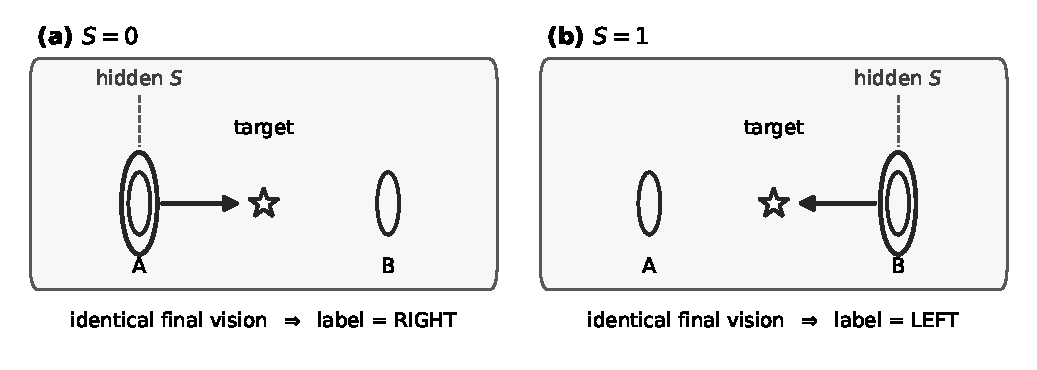
\includegraphics[width=0.92\textwidth]{figures/self_pointer_counterfactual.pdf}
\caption{Same final layout, opposite hidden self ($S=0$ vs.\ $S=1$) and opposite labels. Vision alone cannot tell the rows apart; internal cues during identification are necessary for above-chance performance.}
\label{fig:counterfactual}
\end{figure}

\subsection{Cue ablations}

\begin{description}
\item[Vision only.] Chance control.
\item[Orienting.] One-bit organism-centered response; main test of the motivating hypothesis.
\item[Efference copy.] Self body's motor command; identity requires matching command to motion.
\item[Proprioception.] Self body's displacement; identity requires matching to a visible trajectory.
\item[Explicit self.] Direct one-hot identity; oracle upper bound.
\end{description}

Combinations (orienting+efference, orienting+proprioception, all internal) test whether different cues compress into one latent $Z_t$ rather than isolated shortcuts.

\subsection{Model and training}

Visual tokens are encoded by a small transformer; cues and pooled perception feed a GRU bottleneck $Z_t$. On the next step, $Z_{t-1}$ can recirculate into each object token:
\begin{equation}
\widetilde H_{t,i} = H^{(1)}_{t,i} + \tanh(W_gH^{(1)}_{t,i}) \odot W_zZ_{t-1},
\label{eq:recirc}
\end{equation}
then a second encoder. No hard-coded self slot. Variants disable recirculation, direct $Z$-to-policy readout, or use both.

Training minimizes cross-entropy on the final left/right action only; $S$ is never a target. The useful computation is compositional: $(\text{flash/body relation}, r_t) \rightarrow \widehat S \rightarrow (\widehat S, \text{geometry}) \rightarrow Y$. Explicit self learns fast because the oracle removes discovery; indirect cues show delayed transitions.

\section{Results}

Models use AdamW ($3\times10^{-4}$), horizon eight, 48-d tokens, 32-d $Z$, ``both'' architecture unless noted. Figure~\ref{fig:learning-curves} shows mean held-out accuracy over ten seeds (300 updates, eval every ten rounds, 256 held-out worlds; $\pm 1$ std shaded).

\begin{figure}[t]
\centering
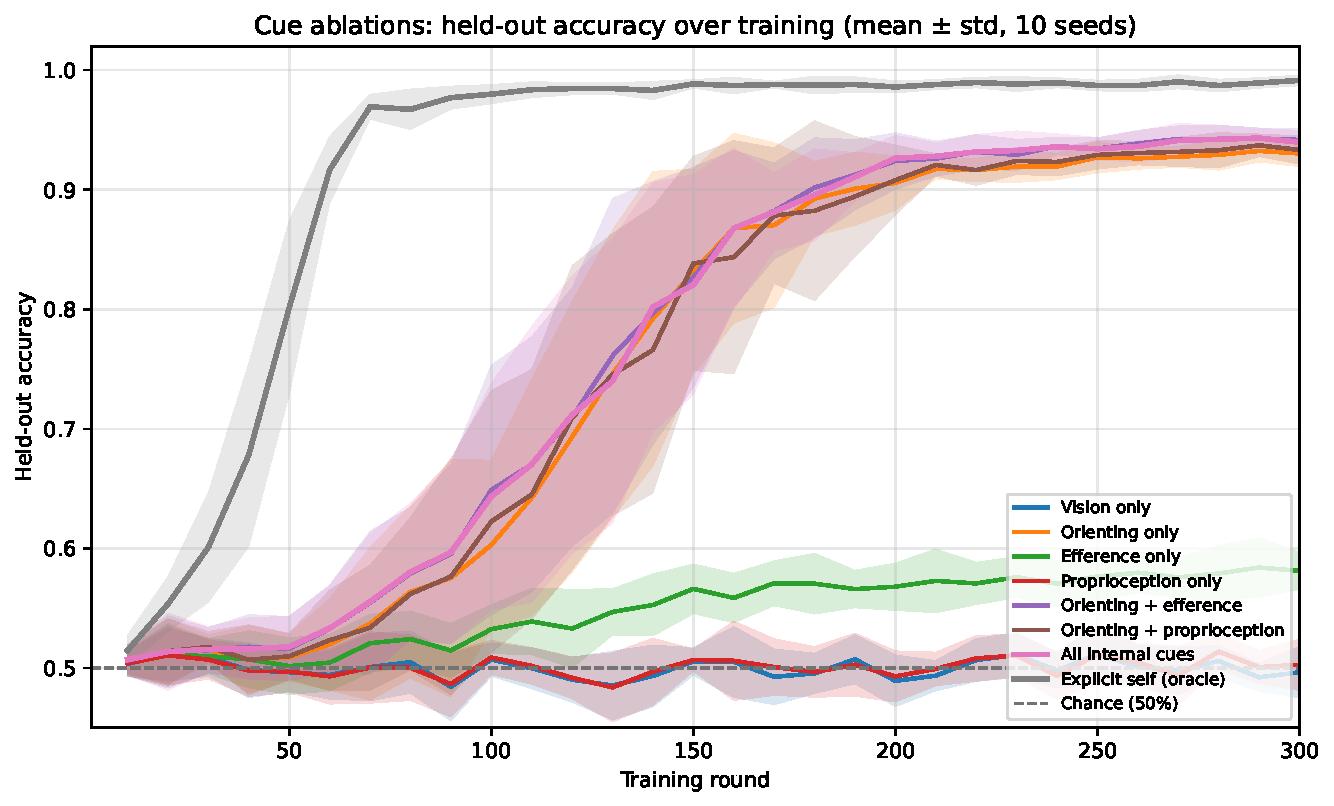
\includegraphics[width=\textwidth]{figures/ablation_learning_curves.pdf}
\caption{Cue ablations (ten seeds). Vision and proprioception stay near chance. Orienting-related conditions transition sharply after $\sim$60--90 rounds. Combinations lead orienting alone slightly at round 300; bands overlap.}
\label{fig:learning-curves}
\end{figure}

Table~\ref{tab:pilot} gives accuracy at round 300. Four takeaways:

\paragraph{Controls work.} Vision ($49.6 \pm 2.1\%$) and proprioception ($50.3 \pm 2.2\%$) stay at chance---symmetry holds, and proprio alone does not solve binding in this horizon.

\paragraph{Orienting learns, slowly.} Orienting-only rises from $60.3 \pm 7.1\%$ (round 100) to $93.0 \pm 1.1\%$ (round 300), well below the oracle decoder. The bottleneck is learning the relation, not cue strength.

\paragraph{Combinations help early, slightly at the end.} At round 100, all-internal ($64.3 \pm 9.5\%$) beats orienting-only ($60.3 \pm 7.1\%$), with large seed variance during the transition. At round 300, combinations reach $93$--$94\%$ vs.\ $93.0 \pm 1.1\%$ for orienting alone---a modest mean advantage with overlapping bands, not a reliable dominance claim.

\paragraph{Single-seed plots mislead.} Variance is wide between rounds $\approx 80$ and $200$; aggregate over seeds before comparing conditions.

\begin{table}[t]
\centering
\caption{Held-out accuracy at training round 300 (mean $\pm$ std, ten seeds). Chance is 50\%.}
\label{tab:pilot}
\begin{tabular}{lc}
\toprule
Condition & Accuracy at round 300 \\
\midrule
Explicit self & $99.1 \pm 0.4$\% \\
Orienting + efference & $94.2 \pm 1.0$\% \\
All internal cues & $94.0 \pm 1.0$\% \\
Orienting + proprioception & $93.3 \pm 1.2$\% \\
Orienting only & $93.0 \pm 1.1$\% \\
Efference only & $58.1 \pm 1.5$\% \\
Proprioception only & $50.3 \pm 2.2$\% \\
Vision only & $49.6 \pm 2.1$\% \\
\bottomrule
\end{tabular}
\end{table}

We have not yet reported multi-seed probe or swap results at the same rigor. The next step is mechanistic readout at fixed checkpoints: does self information appear in $Z$ first, then in object tokens under recirculation, and does patching $Z$ transfer which body the policy treats as self?

\section{Discussion}

The experiment shows that orienting-related cues can support self-relative action in a setting where vision cannot. That is not yet proof of a self-pointer in the stronger sense---a reusable, causally operative, optionally perception-bound latent. Accuracy is the entry ticket; probes and swaps are the test.

The setup separates questions that are entangled in biological data. We can symmetricize vision, ablate cues independently, force retention across a cue-free gap, toggle recirculation, and transplant state between counterfactual twins. Local agency attribution---matching one cue to one body---is the precursor, not the full phenomenon. The interesting claim is \emph{convergence}: efference, proprioception, and orienting compressed into one latent reused across decisions. Cue substitution across episodes would test that directly.

This is not a consciousness experiment. Success would show only a ingredient several theories need implicitly: a world model can learn \emph{which body is mine} from privileged causal relations, not from an external ``self'' symbol. Recursive self-models still need that index \citep{zarncke2025}; organism-centered signals may supply it before recursion builds phenomenology. The thalamic story can be true without making thalamus a consciousness center.

\paragraph{Limitations.}
(1) A pointer is not a phenomenal self---no affect, introspection, or report. (2) Probes can find information the policy ignores; swaps matter. (3) Object-centric inputs simplify perception; pixels and variable agent counts remain open. (4) Supervised final-action training is clean but not developmental; RL may change what latents emerge.

\section{Conclusion}

Two identical bodies, one source of internal signals, opposite actions required---that is the whole puzzle stripped bare. Under matched counterfactuals, orienting-related cues let a small recurrent network learn self-relative control after a delayed transition; vision cannot. Whether the network learns a genuine self-pointer---decodable, swappable, bound into perception---is the open mechanistic question. Either way, the paradigm makes that question empirical.

\bibliographystyle{plainnat}
\bibliography{self-pointers}

\end{document}
